\documentclass[12pt, letterpaper]{../assignment}
\usepackage{graphicx}
\usepackage{courier}
\usepackage{minted}
\usepackage{amsmath}
\usepackage{commath}
\usepackage{amssymb}
\usepackage{amsfonts} 
\usepackage{cancel}
\usepackage{enumitem}
\usepackage{array}

\usepackage{tikz}
\usetikzlibrary{shapes,arrows,positioning}

\usemintedstyle{monokai}
\oddsidemargin = 0pt
\exercisesheet{Module 11}{Practice Assignment}
\student{Austin Barrilleaux}
\courselabel{EN 525.609}
\semester{Fall 2023}
\usepackage[backend=bibtex,style=numeric,sorting=none]{biblatex}
\bibliography{reference}
\usepackage{color}
\definecolor{light-gray}{rgb}{0.2,0.2,0.2}
\setminted{bgcolor=light-gray}
\setlength{\parindent}{0pt}

\makeatletter
\patchcmd{\minted@colorbg}{\noindent}{\medskip\noindent}{}{}
\apptocmd{\endminted@colorbg}{\par\medskip}{}{}
\makeatother

\begin{document}
\subsection*{Problem 1}

\subsubsection*{Solve the following 9th Edition textbook problems:\\
\begin{itemize}
    \item 9-1
    \item 9-43
\end{itemize}}

\subsubsection*{(9-1) The block diagram of a control system with a series controller below.}

\begin{figure}[H]
    \centering
    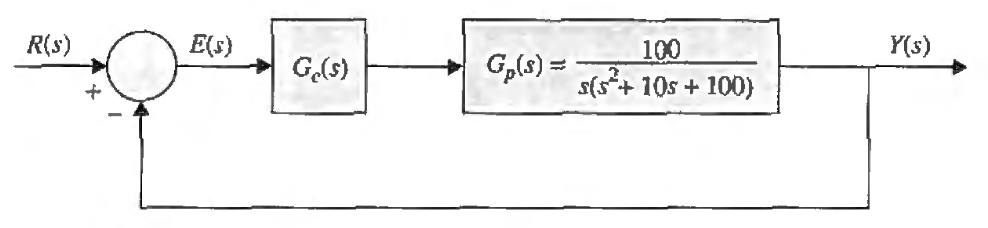
\includegraphics[width=0.85\linewidth]{./figures/Problem_9_1.png}
 \end{figure}

\subsubsection*{Find the transfer function of the controller $\mathbf{G_c(s)}$ so that the following specifications are satisfied:
\begin{itemize}
    \item The ramp error constant $\mathbf{K_v}$ is 5.
    \item The closed-loop transfer function is of the form:
\end{itemize}
$$ \mathbf{ M(s) = \frac{Y(s)}{R(s)} = \frac{K}{(s^2 + 20s + 200)(s+a)} } $$
where $\mathbf{K}$ and $\mathbf{a}$ are real constants.
Find the values of $\mathbf{K}$ and $\mathbf{a}$.}

We know that the closed-loop transfer function is:

$$ M(s) = \frac{G(s)}{1+G(s)} = \frac{K}{(s^2 + 20s + 200)(s+a)} $$

Solving for $G(s)$:

$$ G(s) = \frac{M(s)}{1-M(s)} =  \frac{K}{s^3 + (20 + a)s^2 + (200 + 20a)s + 200a  - K} $$

For this system to have a constant ramp error, the system must be type 1,
so in order to have a zero pole:

$$ 200 a - K = 0 \ \ \ \rightarrow \ \ \ K = 200 a $$

So $G(s)$ becomes:

$$ G(s) = \frac{M(s)}{1-M(s)} =  \frac{200a}{s^3 + (20 + a)s^2 + (200 + 20a)s} $$

The ramp error constant is computed as:

$$ K_v = \lim_{s \to 0} s G(s) = \frac{s \cdot 200a}{s^3 + (20 + a)s^2 + (200 + 20a)s} = \frac{200a}{s^2 + (20 + a)s + (200 + 20a)} $$

Evaluating this:

$$ K_v = \frac{200a}{\cancelto{0}{s^2} + \cancelto{0}{(20 + a)s} + (200 + 20a)} = \frac{200a}{200 + 20a} = 5 $$

\begin{answer}
Solving for $a$, $a = 10$ and $K = 2000$.
\end{answer}


From this we can solve for the transfer function of the controller, $G_c(s)$:

$$ G(s) = G_c(s) G_p(s) \ \ \ \rightarrow \ \ \ G_c(s) = \frac{G(s)}{G_p(s)} $$

So:

$$ G_c(s) = \frac{2000}{s(s^2 + 20s + 400)}
     \left( \frac{s(s^2 + 10s + 100)}{100} \right)$$

$G_c(s)$ reduces to:

\begin{answer}
$$ G_c(s) = \frac{20(s^2 + 10s + 100)}{(s^2 + 20s + 400)} $$
\end{answer}

\subsubsection*{The design strategy is to place the closed-loop poles at $\mathbf{- 10 + j10}$ and $\mathbf{-10 - j10}$,
and then adjust the values of $\mathbf{K}$ and $\mathbf{a}$ to satisfy the steady-state requirement.
The value of $\mathbf{a}$ is large so that it will not affect the transient response appreciably.
Find the maximum overshoot of the designed system.}

\begin{answer}
We can determine the maximum overshoot of the system by using the \texttt{stepinfo()} function in MATLAB.
Doing so, gives us a \textbf{maximum overshoot} of $0$.
\end{answer}

If we plot the response we can see that there is no overshoot:

\begin{figure}[H]
    \centering
    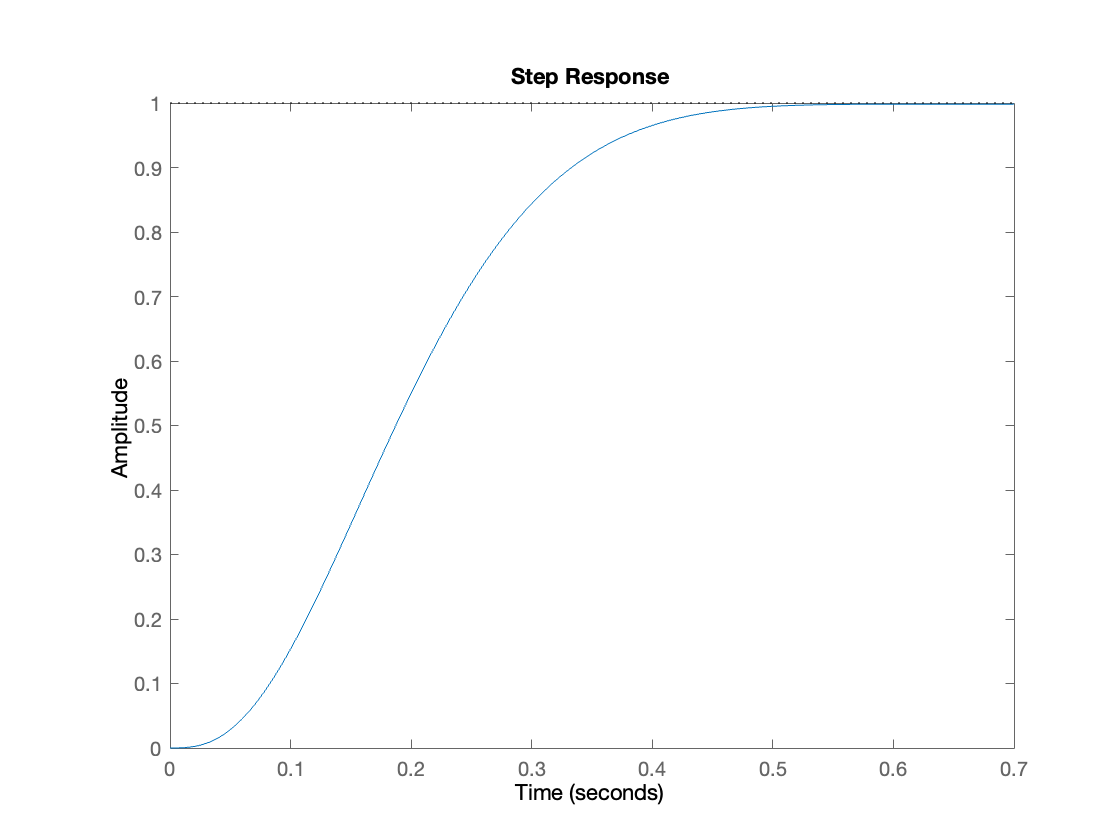
\includegraphics[width=0.85\linewidth]{./figures/step_repsonse.png}
\end{figure}

\subsubsection*{(9-43) Consider that the process of a unity-feedback control system is:}

$$ \mathbf{G_p(s) = \frac{1000}{s(s+10)} } $$

\subsubsection*{Let the series controller be a single-stage phase-lead controller:}

$$ \mathbf{G_c(s) = \frac{1+a T s}{1 + T s} , \ \ a > 1 } $$

\subsubsection*{(a) Determine the values of $\mathbf{a}$ and $\mathbf{T}$ so that the zero of $\mathbf{G_c(s)}$ cancels the pole of $\mathbf{Gp(s)}$ at $\mathbf{s = -10}$.
The damping ratio of the designed system should be unity.
Find the attributes of the unit-step response of the designed system.}

Combining $G_p(s)$ and $G_c(s)$:

$$ G(s) = \frac{1000a (\frac{1}{Ta}+ s)}{s(s+10)(\frac{1}{T} +s)} $$

To cancel the $(s+10)$ pole:

$$ \frac{1}{Ta} = 10 $$

The transfer function becomes:

$$ G(s) = \frac{1000a}{s(\frac{1}{T} +s)}, \ \ \frac{1}{Ta} = 10 $$

The characteristic equation of the closed loop transfer function is:

$$ s^2 + \frac{s}{T} + 1000a = 0 $$

From this, we can define $\zeta$ and $\omega_n$ as:

$$ \frac{1}{T} = 2 \zeta \omega_n \ \ \ \omega_n = \sqrt{1000a}  $$

Therefore:

$$ \frac{1}{T} = 10a = 2 \zeta \omega_n = 2 \sqrt{1000a} $$

\begin{answer}
    $$ 100a^2 = 4000a \ \ \rightarrow  \ \ a = 40 $$
\end{answer}

\begin{answer}
    $$ T = \frac{1}{10a} = \frac{1}{400} $$
\end{answer}

\begin{answer}
    The constant $a = 40$ and $T = 0.0025$.
\end{answer}

The closed loop transfer function is:

$$ M(s) = \frac{40000}{s^2 + 400s + 40000} $$

Solvinf for the attributes of the system:
$$ \zeta = \frac{400}{2 \omega_n}  =\frac{400}{2 \sqrt{40000}} = 1 $$

\begin{answer}
Therefor, maximum overshoot is $0$.
\end{answer}

The rise time can be approximated as:

\begin{answer}
$$ t_r = \frac{0.8+2.5\zeta}{\omega_n} = 0.0165 \ \  \text{sec} $$
\end{answer}

The settling time can be approximated as:

\begin{answer}
$$ t_s = \frac{4.5 \zeta}{\omega_n} = 0.0225\ \  \text{sec}, \ \ \ \zeta > 0.69 $$
\end{answer}

\subsubsection*{(b) Carry out the design in the frequency domain using the Bode plot. The design specifications are as follows:\\
\begin{itemize}
    \item Phase margin $\mathbf{> 75^\circ}$
    \item $\mathbf{M_r < 1.1}$
\end{itemize}
Find the attributes of the unit-step response of the designed system.}

The uncompensated open loop transfer function is:

$$ G (s) = \frac{1000}{s(s+10)} $$

The attributes of the system using \texttt{margin()} and \texttt{getPeakMargin()} functions in MATLAB,
we see that $PM = 17.9642$, $GM = \infty$ and $M_r = 3.2026$
\\\\
In order the meet the phase margin requirement, we need to shift it by:

$$ 75^\circ-17.9642^\circ+15^\circ = 72.0358^\circ$$

This includes a fudge factor of $5^\circ$.
\\\\
$a$ is calculated as:

$$ a = \frac{1+\sin(72.0358^\circ)}{1-\sin(72.0358^\circ)} = 40.0251 $$

The gain of the controller is calculated as:

$$ -10 \log_{10} (a) = -10 \log_{10} (40.0251) = -16.0233 \ \text{dB} $$

The gain magnitude is:

$$ |G(j\omega)| = \left| \frac{1000}{j\omega(j\omega+100)} \right| 
    = \frac{1000}{\omega \sqrt{\omega^2+100} }  $$

We can solve for the new gain crossover frequency as:

$$ \frac{1000}{\omega \sqrt{\omega^2+10}} = 10^{\frac{-16.0233 }{20}} $$

We can put this in the form:

$$ \omega^4 + 100\omega^2 + \left(\frac{1000}{10^{\frac{-16.0233 }{20}}}\right)^2 = 0 $$

We can solve for $\omega_\text{max}$ via the following:

$$ \omega_\text{max} = \sqrt{-10+\sqrt{10^2 + \left(\frac{1000}{10^{\frac{-16.0233 }{20}}}\right)^2}}
    = 79.4767 \ \text{rad/s} $$

The relationship between $\omega_\text{max}$ and the compensator pole / zero location is:

$$ \omega_\text{max} = \frac{1}{\tau \sqrt{a}} = \frac{1}{T \sqrt{a}} \ \ ,
    \ \ \ \ \ \ \ \ \  (\tau = T) $$

Therefore:

$$ T = \frac{1}{\sqrt{a} \omega_\text{max}} = 0.0020 \ \text{rad/s} $$

The controller transfer function is:

$$ G_c(s) = \frac{1+0.0796 s}{1 + 0.0020s} $$

We now get the following for $G(s)$:

$$ G(s) = \frac{1000}{s(s+10)}\left(\frac{1+0.0796 s}{1 + 0.0020s}\right)
    =  \frac{79.6 s + 1000}{0.001989 s^3 + 1.02 s^2 + 10 s} $$

\begin{answer}
    If we evaluate this using the \texttt{margin()} function in MATLAB,
    we get that $PM = 79.2502$ and $GM = \infty$.
\end{answer}

\begin{answer}
    If we evaluate it's corresponding closed loop transfer function using the \texttt{getPeakMargin()} function in MATLAB,
    we get that $M_r= 1.0096$.
\end{answer}

\begin{answer}
This controller design satisfies both of the constraints, that $\mathbf{PM > 75^\circ}$ and $\mathbf{M_r < 1.1}$.
\end{answer}

The attributes of the unit-step response of the designed system,
found using the \texttt{stepinfo()} function in MATLAB are:

\begin{answer}
\begin{itemize}
\item $t_r = 0.0216$ sec
\item $t_s = 0.0348$ sec
\item \textbf{\%OS} $= 1.7075$ \%
\end{itemize} 
\end{answer}

The step response can be seen here:

\begin{figure}[H]
    \centering
    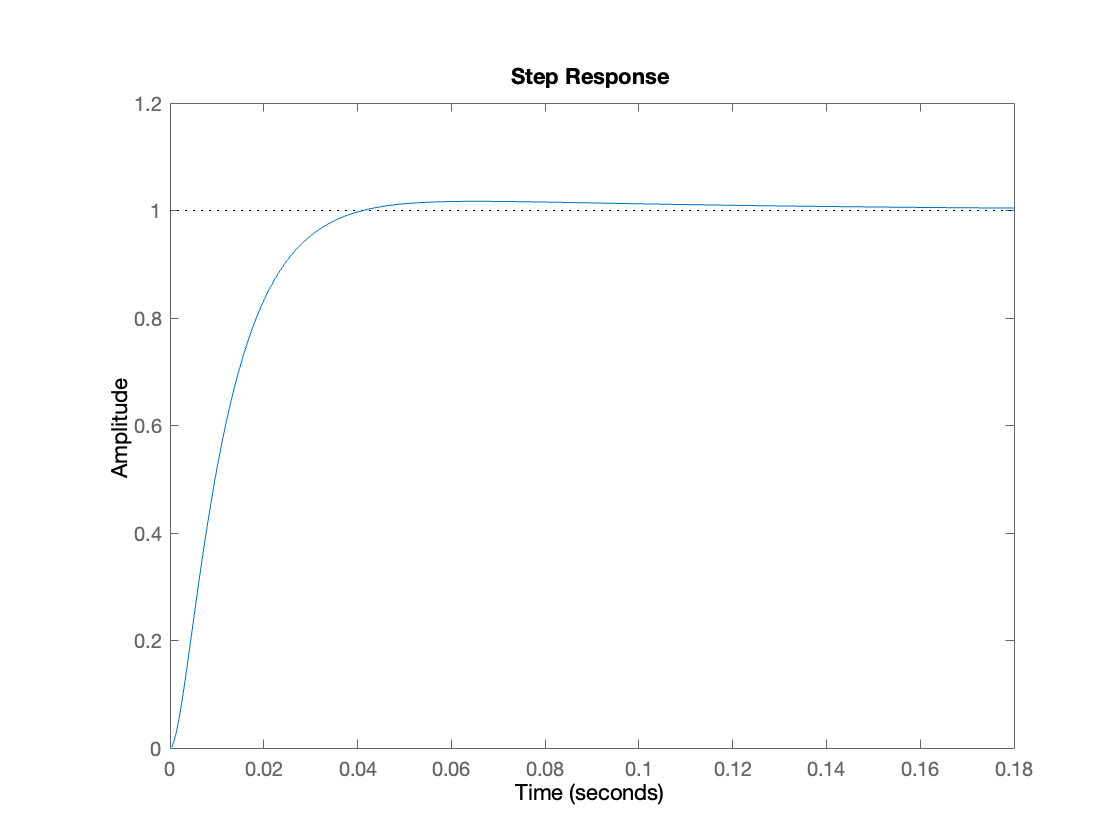
\includegraphics[width=0.85\linewidth]{./figures/step_repsonse_designed_controller.png}
\end{figure}

The bode plot for the system is:

\begin{figure}[H]
    \centering
    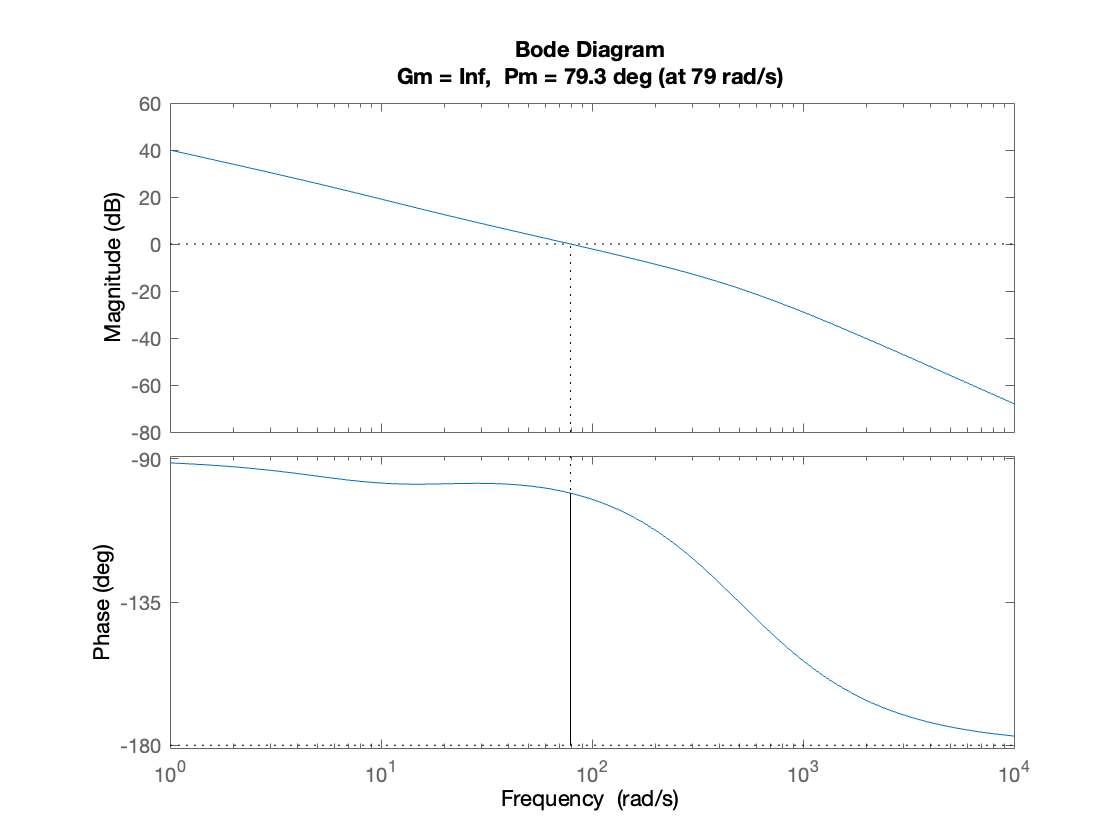
\includegraphics[width=0.85\linewidth]{./figures/margin_plot.png}
\end{figure}

I attempted this part the first time with a fudge factor of $5^\circ$,
which did not meet the design requirements.

% \color{white}
% \hspace*{6em}\inputminted[frame=leftline,fontsize=\footnotesize]{matlab}
% {./matlab/Problem_5_18.m}
% \color{black}

% \begin{figure}[H]
%     \centering
%     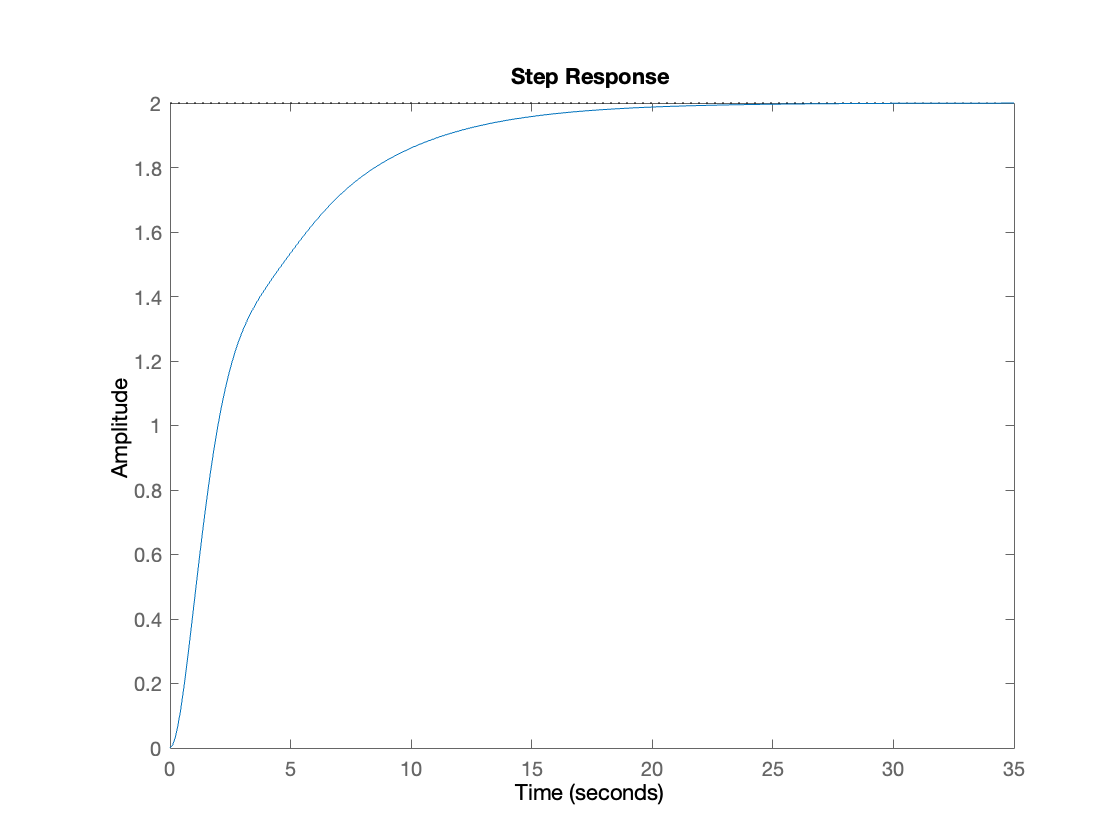
\includegraphics[width=0.7\linewidth]{./figures/step_response.png}
%     \caption{Step Response}
%     \label{fig:step}
%  \end{figure}



\end{document}

